\let\negmedspace\undefined
\let\negthickspace\undefined
\documentclass[journal]{IEEEtran}
\usepackage[a5paper, margin=10mm, onecolumn]{geometry}
%\usepackage{lmodern} % Ensure lmodern is loaded for pdflatex
\usepackage{tfrupee} % Include tfrupee package

\setlength{\headheight}{1cm} % Set the height of the header box
\setlength{\headsep}{0mm}     % Set the distance between the header box and the top of the text

\usepackage{gvv-book}
\usepackage{gvv}
\usepackage{cite}
\usepackage{amsmath,amssymb,amsfonts,amsthm}
\usepackage{algorithmic}
\usepackage{graphicx}
\usepackage{textcomp}
\usepackage{xcolor}
\usepackage{txfonts}
\usepackage{listings}
\usepackage{enumitem}
\usepackage{mathtools}
\usepackage{gensymb}
\usepackage{comment}
%\usepackage{multiclo}
\usepackage[breaklinks=true]{hyperref}
\usepackage{tkz-euclide} 
\usepackage{listings}
% \usepackage{gvv} 
\graphicspath{ {./figs/} }

\begin{document}

\title{
ME: MECHANICAL ENGINEERING}
\author{AI25BTECH11011}
\maketitle
\renewcommand{\thefigure}{\theenumi}
\renewcommand{\thetable}{\theenumi}

\textbf{Q.1 - Q.5 carry one mark each.}

\begin{enumerate}

\item Choose the appropriate word/phrase to complete the sentence:

Dhoni, as well as the other team members of Indian team, ----------- present on the occasion.
\begin{multicols}{4}
\begin{enumerate}
\item were  
\item was  
\item has  
\item have  
\end{enumerate}
\end{multicols}
\hfill  (GATE ME 2015)

\item Choose the word most similar in meaning to:

\textbf{Awkward}
\begin{multicols}{4}
\begin{enumerate}
\item Inept  
\item Graceful  
\item Suitable  
\item Dreadful  
\end{enumerate}
\end{multicols}
\hfill  (GATE ME 2015)

\item What is the adverb for the given word below?

\textbf{Misogynous}
\begin{multicols}{4}
\begin{enumerate}
\item Misogynousness  
\item Misogynity  
\item Misogynously  
\item Misogynous  
\end{enumerate}
\end{multicols}
\hfill  (GATE ME 2015)


\item An electric bus has onboard instruments that report the total electricity consumed since the start of the trip as well as the total distance covered. During a single day of operation, the bus travels on stretchs M,N,O and P, in that order. The \underline{cumulative} distances travelled and the corresponding electricity are shown in the Table below:

\begin{tabular}{|c|c|c|}
\hline
 Stretch & Cumulative distance (km) & Electricity used (kWh) \\
 M & 20 & 12 \\
 \hline
 N & 45 & 25 \\
 \hline
 O & 75 & 45 \\
 \hline
 P & 100 & 57 \\
\hline
\end{tabular}


The stretch where the electricity consumption per km is minimum is
\begin{multicols}{4}
\begin{enumerate}
\item M  
\item N  
\item O  
\item P  
\end{enumerate}
\end{multicols}
\hfill  (GATE ME 2015)

\item Ram and Ramesh appeared in an interview for two vacancies in the same department. The probability of Ram's selection is $ \frac{1}{6} $ and that of Ramesh is $ \frac{1}{8} $. What is the probability that only one of them will be selected?
\begin{enumerate}
\item $ \frac{47}{48} $  
\item $ \frac{1}{4} $  
\item $ \frac{13}{48} $  
\item $ \frac{35}{48} $  
\end{enumerate}
\hfill  (GATE ME 2015)

\textbf{Q.6 - Q.10 carry two marks each.}

\item In the following sentence, certain parts are underlined and marked P, Q, and R. One of the parts may contain an error or may not be acceptable in standard written communication. Select the part containing an error. Choose (D) as your answer if there is no error.

 The student corrected \underline{all the errors} that \underline{the instructor marked} on the \underline{answer book}.

\hfill P \hfill Q \hfill R
\begin{multicols}{4}
\begin{enumerate}
\item P  
\item Q  
\item R  
\item No Error  
\end{enumerate}
\end{multicols}
\hfill  (GATE ME 2015)

\item Given below are two statements followed by two conclusions. Assuming these statements to be true, decide which one logically follows.

Statements:  

I. All film stars are playback singers. 

II. All film directors are film stars. 

Conclusions: 

I. All film directors are playback singers.

II. Some film stars are film directors.

\begin{enumerate}
\item Only conclusion I follows  
\item Only conclusion II follows  
\item Neither follows  
\item Both follow  
\end{enumerate}
\hfill  (GATE ME 2015)

\item A tiger is 50 leaps behind a deer. Tiger: 5 leaps/min, 8 m/leap. Deer: 4 leaps/min, 5 m/leap. Distance tiger runs before catching deer?  

\textbf{Answer:} 
\hfill  (GATE ME 2015)

\item If $ a^2 + b^2 + c^2 = 1 $, then $ ab + bc + ac $ lies in the interval:

\begin{enumerate}
\item $ [1, \frac{2}{3}] $  
\item $ [-\frac{1}{2}, 1] $  
\item $ [-1, \frac{1}{2}] $  
\item $ [2, -4] $    
\end{enumerate}
\hfill  (GATE ME 2015)

\item Lamenting the gradual sidelining of the arts in school curricula, a group of prominent artists wrote to the Chief Minister last year, asking him to allocate more funds to support arts education in schools. However, no such increase has been announced in this year's Budget. The artists expressed their deep anguish at their request not being approved, but many of them remain optimistic about funding in the future.

Which of the statement(s) below is/are logically valid and can be inferred from the above statements?

\begin{enumerate}[label=(\roman*)]
\item The artists expected funding for the arts to increase this year.  
\item The Chief Minister was receptive to the idea of increasing funding for the arts.  
\item The Chief Minister is a prominent artist.  
\item Schools are giving less importance to arts education nowadays.  
\end{enumerate}

\begin{multicols}{2}
\begin{enumerate}
\item (iii) and (iv)  
\item (i) and (iv)  
\item (i), (ii) and (iv)  
\item (i) and (iii)  
\end{enumerate}
\end{multicols}
\hfill  (GATE ME 2015)

\textbf{Q.11 - Q.35 carry one mark each.}

\item If any two columns of a determinant 
$\Vec{p} = \myvec{4 & 7 & 8 \\
                  3 & 1 & 5 \\
                  9 & 6 & 2 }$
are interchanged, which one of the following statements regarding the value of the determinant is CORRECT?
\begin{enumerate}
\item Absolute value remains unchanged but sign will change.  
\item Both absolute value and sign will change.  
\item Absolute value will change but sign will not change.  
\item Both absolute value and sign will remain unchanged.  
\end{enumerate}
\hfill  (GATE ME 2015)

\item Among the four normal distributions with probability density functions as shown below, which one has the lowest variance?

\begin{figure}[H]
    \centering
    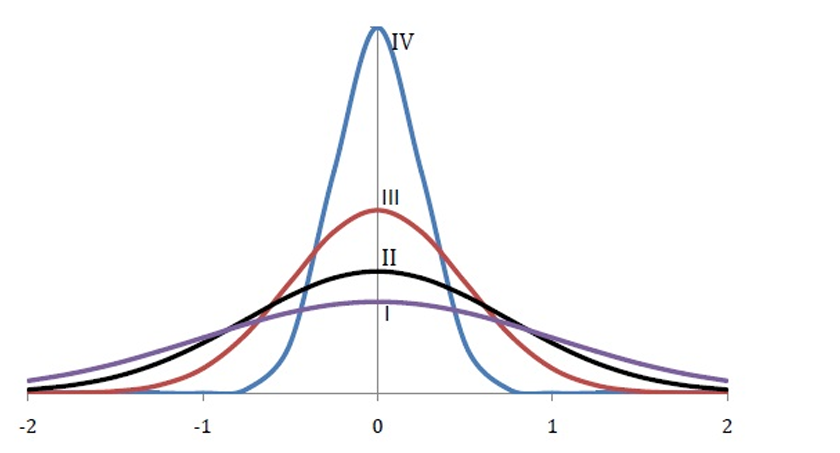
\includegraphics[width=0.8\textwidth]{Fig 1.png}
    \caption{}
    \label{fig:question12}
\end{figure}

\begin{multicols}{4}
\begin{enumerate}
\item I  
\item II  
\item III  
\item IV  
\end{enumerate}
\end{multicols}
\hfill  (GATE ME 2015)

\item Simpson’s $\tfrac{1}{3}$ rule is used to integrate the function
$f(x)=\tfrac{3}{5}x^{2}+\tfrac{9}{5}$ between $x=0$ and $x=1$ using the
least number of equal sub-intervals. The value of the integral is ----------.
\hfill  (GATE ME 2015)

\item The value of $\displaystyle \lim_{x\to 0}\frac{1-\cos\!\left(x^{2}\right)}{2x^{4}}$ is
\begin{multicols}{2}
\begin{enumerate}
\item $0$
\item $\tfrac{1}{2}$
\item $\tfrac{1}{4}$
\item undefined
\end{enumerate}
\end{multicols}
\hfill  (GATE ME 2015)

\item Given two complex numbers $z_{1}=5+(5\sqrt{3})i$ and $z_{2}=\tfrac{2}{\sqrt{3}}+2i$,
the argument of $\tfrac{z_{1}}{z_{2}}$ in degrees is
\begin{multicols}{4}
\begin{enumerate}
\item $0$
\item $30$
\item $60$
\item $90$
\end{enumerate}
\end{multicols}
\hfill  (GATE ME 2015)

\item Consider fully developed flow in a circular pipe with negligible entrance length effects.
Assuming the mass flow rate, density and friction factor to be constant, if the length of the
pipe is doubled and the diameter is halved, the head loss due to friction will increase by a factor of
\begin{multicols}{4}
\begin{enumerate}
\item $4$
\item $16$
\item $32$
\item $64$
\end{enumerate}
\end{multicols}
\hfill  (GATE ME 2015)

\item The Blasius equation related to boundary layer theory is a
\begin{enumerate}
\item third-order linear partial differential equation
\item third-order nonlinear partial differential equation
\item second-order nonlinear ordinary differential equation
\item third-order nonlinear ordinary differential equation
\end{enumerate}
\hfill  (GATE ME 2015)

\item For flow of viscous fluid over a flat plate, if the fluid temperature is the same as the plate
temperature, the thermal boundary layer is
\begin{enumerate}
\item thinner than the velocity boundary layer
\item thicker than the velocity boundary layer
\item of the same thickness as the velocity boundary layer
\item not formed at all
\end{enumerate}
\hfill  (GATE ME 2015)

\item For an ideal gas with constant values of specific heats, for calculation of the specific enthalpy,
\begin{enumerate}
\item it is sufficient to know only the temperature
\item both temperature and pressure are required to be known
\item both temperature and volume are required to be known
\item both temperature and mass are required to be known
\end{enumerate}
\hfill  (GATE ME 2015)

\item A Carnot engine (CE-1) works between two temperature reservoirs A and B, where $T_{A}=900\ \mathrm{K}$ and
$T_{B}=500\ \mathrm{K}$. A second Carnot engine (CE-2) works between temperature reservoirs B and C, where
$T_{C}=300\ \mathrm{K}$. In each cycle of CE-1 and CE-2, all the heat rejected by CE-1 to reservoir B is used by CE-2.
For one cycle of operation, if the net $Q$ absorbed by CE-1 from reservoir A is $150\ \mathrm{MJ}$, the net heat rejected
to reservoir C by CE-2 (in MJ) is ------------.
\hfill  (GATE ME 2015)

\item Air enters a diesel engine with a density of $1.0\ \mathrm{kg/m^{3}}$. The compression ratio is $21$.
At steady state, the air intake is $30\times 10^{-3}\ \mathrm{kg/s}$ and the net work output is $15\ \mathrm{kW}$.
The mean effective pressure (in kPa) is ------------.
\hfill  (GATE ME 2015)

\item A stream of moist air (mass flow rate $=10.1\ \mathrm{kg/s}$) with humidity ratio of
$0.01\ \dfrac{\mathrm{kg}}{\mathrm{kg\ dry\ air}}$ mixes with a second stream of superheated water vapour flowing at
$0.1\ \mathrm{kg/s}$. Assuming proper and uniform mixing with no condensation, the humidity ratio of the final stream
$\left(\ \dfrac{\mathrm{kg}}{\mathrm{kg\ dry\ air}}\ \right)$ is -----------.
\hfill  (GATE ME 2015)

\item A wheel of radius $r$ rolls without slipping on a horizontal surface shown below. If the velocity of point $P$
is $10\ \mathrm{m/s}$ in the horizontal direction, the magnitude of velocity of point $Q$ (in m/s) is ------------.
\begin{figure}[H]
    \centering
    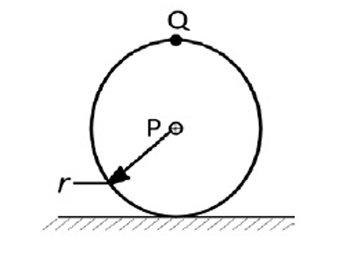
\includegraphics[width=0.8\textwidth]{Fig 2.png}
    \caption{}
    \label{fig:question23}
\end{figure}
\hfill  (GATE ME 2015)

\item Consider a slider crank mechanism with nonzero masses and inertia. A constant torque $\tau$ is applied on the
crank as shown in the figure. Which of the following plots best resembles variation of crank angle, $\theta$ versus time?

\begin{figure}[H]
    \centering
    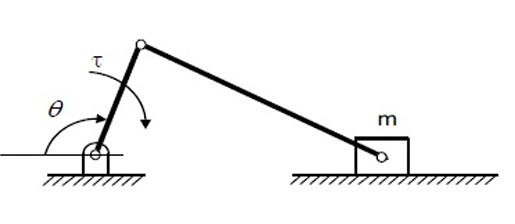
\includegraphics[width=0.8\textwidth]{Fig 3.png}
    \caption{}
    \label{fig:question24}
\end{figure}

\begin{enumerate}

\item \begin{figure}[H]
    \centering
    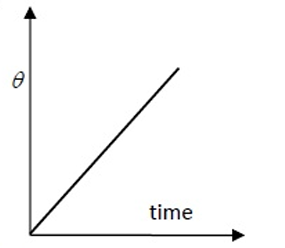
\includegraphics[width=0.2\textwidth]{Fig 4.png}
    \caption{}
    \label{fig:question24}
\end{figure}

\item \begin{figure}[H]
    \centering
    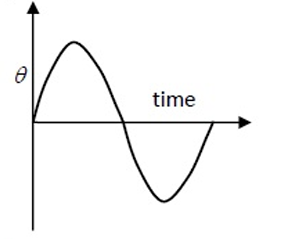
\includegraphics[width=0.2\textwidth]{Fig 5.png}
    \caption{}
    \label{fig:question24}
\end{figure}

\item \begin{figure}[H]
    \centering
    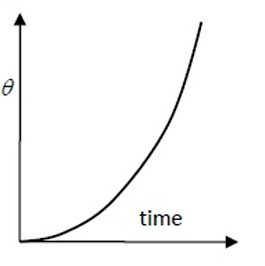
\includegraphics[width=0.2\textwidth]{Fig 6.png}
    \caption{}
    \label{fig:question24}
\end{figure}

\item \begin{figure}[H]
    \centering
    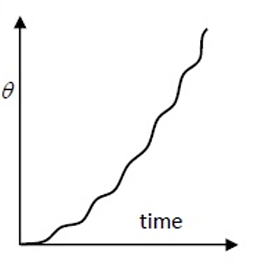
\includegraphics[width=0.2\textwidth]{Fig 7.png}
    \caption{}
    \label{fig:question24}
\end{figure}

\end{enumerate}
\hfill  (GATE ME 2015)

\item Consider a stepped shaft subjected to a twisting moment applied at $B$ as shown in the figure.
Assume shear modulus, $G=77\ \mathrm{GPa}$. The angle of twist at $C$ (in degrees) is --------------.
\begin{figure}[H]
    \centering
    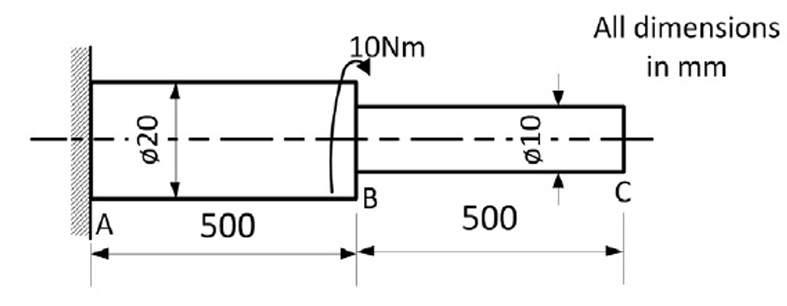
\includegraphics[width=0.8\textwidth]{Fig 8.png}
    \caption{All dimensions in mm}
    \label{fig:question25}
\end{figure}
\hfill  (GATE ME 2015)

\item Two identical trusses support a load of $100\ \mathrm{N}$ as shown in the figure. The length of each truss is $1.0\ \mathrm{m}$; cross-sectional area is $200\ \mathrm{mm}^2$; Young's modulus $E = 200\ \mathrm{GPa}$.  
The force in the truss AB (in N) is --------------.

\begin{figure}[H]
    \centering
    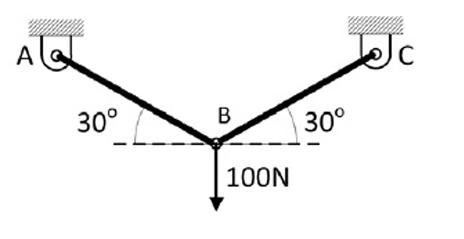
\includegraphics[width=0.8\textwidth]{Fig 9.png}
    \caption{}
    \label{fig:question26}
\end{figure}
\hfill  (GATE ME 2015)

\item Consider a steel column (Young's modulus $E = 200\ \mathrm{GPa}$) hinged at both ends. Its height is $1.0\ \mathrm{m}$ and cross-section is $10\ \mathrm{mm}\times 20\ \mathrm{mm}$.  
The lowest Euler critical buckling load (in N) is --------------.
\hfill  (GATE ME 2015)

\item A swimmer can swim $10\ \mathrm{km}$ in $2$ hours when swimming along the flow of a river. While swimming against the flow, she takes $5$ hours for the same distance.  
Her speed in still water (in km/h) is --------------.
\hfill  (GATE ME 2015)

\item Which one of the following is the most conservative fatigue failure criterion?
\begin{multicols}{2}
\begin{enumerate}
    \item Soderberg
    \item Modified Goodman
    \item ASME Elliptic
    \item Gerber
\end{enumerate}
\end{multicols}
\hfill  (GATE ME 2015)

\item Which one of the following types of stress-strain relationship best describes the behaviour of brittle materials, such as ceramics and thermosetting plastics, ($\sigma = stress$ and $\epsilon = strain$)?

\begin{multicols}{2}
\begin{enumerate}

\item\begin{figure}[H]
    \centering
    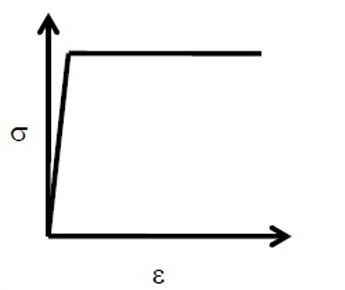
\includegraphics[width=0.3\textwidth]{Fig 10.png}
    \caption{}
    \label{fig:question30}
\end{figure}

\item\begin{figure}[H]
    \centering
    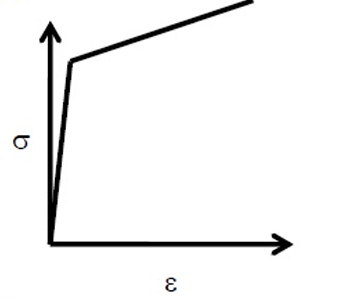
\includegraphics[width=0.3\textwidth]{Fig 11.png}
    \caption{}
    \label{fig:question30}
\end{figure}

\item\begin{figure}[H]
    \centering
    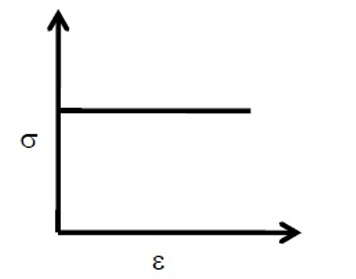
\includegraphics[width=0.3\textwidth]{Fig 12.png}
    \caption{}
    \label{fig:question30}
\end{figure}

\item\begin{figure}[H]
    \centering
    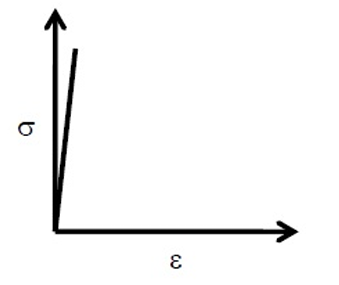
\includegraphics[width=0.3\textwidth]{Fig 13.png}
    \caption{}
    \label{fig:question30}
\end{figure}

\end{enumerate}
\end{multicols}
\hfill  (GATE ME 2015)

\item Match the following products with preferred manufacturing processes:

\begin{tabular}{|c|c|c|c|}
\hline
 & Product              &     & Process \\
\hline
P &  Rails              & 1   &  Blow molding \\
\hline
Q &  Engine crankshaft  & 2   &  Extrusion \\
\hline
R &  Aluminium channels & 3   &  Forging \\
\hline
S &  PET water bottles  & 4   &  Rolling \\
\hline
\end{tabular}

\begin{enumerate}
    \item P-4, Q-3, R-1, S-2
    \item P-4, Q-3, R-2, S-1
    \item P-2, Q-4, R-3, S-1
    \item P-3, Q-4, R-2, S-1
\end{enumerate}
\hfill  (GATE ME 2015)

\item Holes of diameter $ 25.0^{+0.040}_{+0.020} $ mm are assembled interchangeably with the pins of diameter $ 25.0^{+0.005}_{-0.008} $ mm. The minimum clearance in the assembly will be

\begin{enumerate}
    \item 0.048 mm
    \item 0.015 mm
    \item 0.005 mm
    \item 0.008 mm
\end{enumerate}
\hfill  (GATE ME 2015)

\item Under certain cutting conditions, doubling the cutting speed reduces the tool life to $ \left( \frac{1}{16} \right)^{th} $ of the original. Taylor’s tool life index ($ n $) for this tool-workpiece combination will be -------------.
\hfill  (GATE ME 2015)

\item In a linear arc welding process, the heat input per unit length is inversely proportional to

\begin{enumerate}
    \item welding current
    \item welding voltage
    \item welding speed
    \item duty cycle of the power source
\end{enumerate}
\hfill  (GATE ME 2015)

\item The function of interpolator in a CNC machine controller is to

\begin{enumerate}
    \item control spindle speed
    \item coordinate feed rates of axes
    \item control tool rapid approach speed
    \item perform Miscellaneous (M) functions (tool change, coolant control etc.)
\end{enumerate}
\hfill  (GATE ME 2015)

\textbf{Q.36 - Q.65 carry two marks each.}

\item Consider a spatial curve in three-dimensional space given in parametric form by
$x(t) = \cos t, \quad y(t) = \sin t, \quad z(t) = \frac{2}{\pi} t, \quad 0 \leq t \leq \frac{\pi}{2}$

The length of the curve is -------------.
\hfill  (GATE ME 2015)

\item Consider an ant crawling along the curve $(x - 2)^2 + y^2 = 4$, where $x$ and $y$ are in meters. The ant starts at the point $(4, 0)$ and moves counter-clockwise with a speed of 1.57 meters per second. The time taken by the ant to reach the point $(2, 2)$ is (in seconds) -------------.
\hfill  (GATE ME 2015)

\item Find the solution of $ \frac{d^2 y}{dx^2} = y $ which passes through the origin and the point $ (\ln 2, \frac{3}{4}) $.

\begin{enumerate}
    \item $ y = \frac{1}{2} e^x - e^{-x} $
    \item $ y = \frac{1}{2} (e^x + e^{-x}) $
    \item $ y = \frac{1}{2} (e^x - e^{-x}) $
    \item $ y = \frac{1}{2} e^x + e^{-x} $
\end{enumerate}
\hfill  (GATE ME 2015)

\item The probability of obtaining at least two “SIX” in throwing a fair dice 4 times is

\begin{multicols}{4}
\begin{enumerate}
    \item 425/432
    \item 19/144
    \item 13/144
    \item 125/432
\end{enumerate}
\end{multicols}
\hfill  (GATE ME 2015)

\item In the assembly shown below, the part dimensions are:

$L_1 = 22.0 \pm 0.01 \, \text{mm},$

$L_2 = L_3 = 10.0 \pm 0.005 \, \text{mm}.$

Assuming the normal distribution of part dimensions, the dimension $L_4$ in mm for assembly condition would be:

\begin{figure}[H]
    \centering
    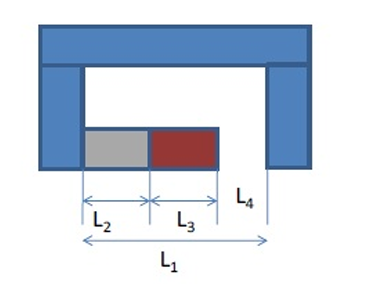
\includegraphics[width=0.8\textwidth]{Fig 14.png}
    \caption{}
    \label{fig:question40}
\end{figure}

\begin{enumerate}
    \item $2.0 \pm 0.008$
    \item $2.0 \pm 0.012$
    \item $2.0 \pm 0.016$
    \item $2.0 \pm 0.020$
\end{enumerate}
\hfill  (GATE ME 2015)

\item A DC welding power source has a linear voltage-current ($V$-$I$) characteristic with open circuit voltage of 80 V and a short circuit current of 300 A. For maximum arc power, the current (in Amperes) should be set as -------------.
\hfill  (GATE ME 2015)

\item A triangular facet in a CAD model has vertices: P1(0,0,0); P2(1,1,0) and P3(1,1,1). The area of the facet is

\begin{enumerate}
    \item 0.500
    \item 0.707
    \item 1.414
    \item 1.732
\end{enumerate}
\hfill  (GATE ME 2015)

\item Following data refers to the activities of a project, where, node 1 refers to the start and node 5 refers to the end of the project.

\begin{tabular}{|c|c|}
\hline
Activity & Duration (days) \\
\hline
1-2 & 2 \\
\hline
2-3 & 1 \\
\hline
4-3 & 3 \\
\hline
1-4 & 3 \\
\hline
2-5 & 3 \\
\hline
3-5 & 2 \\
\hline
4-5 & 4 \\
\hline
\end{tabular}

The critical path (CP) in the network is

\begin{enumerate}
    \item 1-2-3-5
    \item 1-4-3-5
    \item 1-2-3-4-5
    \item 1-4-5
\end{enumerate}
\hfill  (GATE ME 2015)

\item For a canteen, the actual demand for disposable cups was 500 units in January and 600 units in February. The forecast for the month of January was 400 units. The forecast for the month of March considering smoothing coefficient as 0.75 is -------------.
\hfill  (GATE ME 2015)

\item An orthogonal turning operation is carried out under the following conditions: rake angle = $ 5^\circ $; spindle rotational speed = 400 rpm; axial feed = 0.4 m/min and radial depth of cut = 5 mm. The chip thickness, $ t_c $, is found to be 3 mm. The shear angle (in degrees) in this turning process is -------------.
\hfill  (GATE ME 2015)

\item The solidification time of a casting is proportional to $ \left( \frac{V}{A} \right)^2 $, where $ V $ is the volume of the casting and $ A $ is the total casting surface area losing heat. Two cubes of same material and size are cast using sand casting process. The top face of one of the cubes is completely insulated. The ratio of the solidification time for the cube with top face insulated to that of the other cube is

\begin{multicols}{4}
\begin{enumerate}
    \item $ \frac{25}{36} $
    \item $ \frac{36}{25} $
    \item 1
    \item $ \frac{6}{5} $
\end{enumerate}
\end{multicols}
\hfill  (GATE ME 2015)

\item In a slab rolling operation, the maximum thickness reduction $ (\Delta h_{max}) $ is given by $ \Delta h_{max} = \mu^2 R $, where $ R $ is the radius of the roll and $ \mu $ is the coefficient of friction between the roll and the sheet. If $ \mu = 0.1 $, the maximum angle subtended by the deformation zone at the centre of the roll (bite angle in degrees) is -------------.

\hfill  (GATE ME 2015)

\item Considering massless rigid rod and small oscillations, the natural frequency (in rad/s) of vibration of the system shown in the figure is

\begin{figure}[H]
\centering
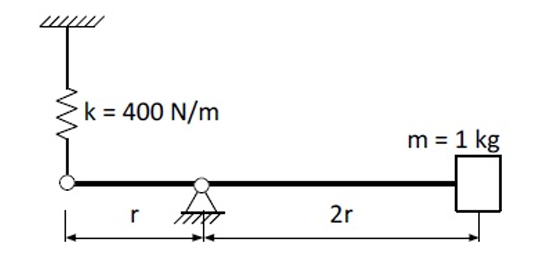
\includegraphics[width=0.8\textwidth]{Fig 15.png}
\caption{}
\label{fig:question48}
\end{figure}

\begin{multicols}{4}
\begin{enumerate}
    \item $\sqrt{\frac{400}{1}}$
    \item $\sqrt{\frac{400}{2}}$
    \item $\sqrt{\frac{400}{3}}$
    \item $\sqrt{\frac{400}{4}}$
\end{enumerate}
\end{multicols}
\hfill  (GATE ME 2015)

\item For the truss shown in figure, the magnitude of the force in member $ PR $ and the support reaction at $ R $ are respectively

\begin{figure}[H]
\centering
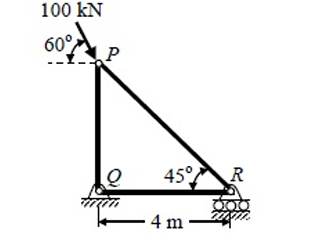
\includegraphics[width=0.5\textwidth]{Fig 16.png}
\caption{}
\label{fig:question49}
\end{figure}

\begin{multicols}{2}
\begin{enumerate}
    \item 122.47 kN and 50 kN
    \item 70.71 kN and 100 kN
    \item 70.71 kN and 50 kN
    \item 81.65 kN and 100 kN
\end{enumerate}
\end{multicols}
\hfill  (GATE ME 2015)

\item A ball of mass 0.1 kg, initially at rest, is dropped from height of 1 m. Ball hits the ground and bounces off the ground. Upon impact with the ground, the velocity reduces by 20\%. The height (in m) to which the ball will rise is -------------.

\hfill  (GATE ME 2015)

\item A pinion with radius $ r_1 $, and inertia $ I_1 $ is driving a gear with radius $ r_2 $ and inertia $ I_2 $. Torque $ \tau_1 $ is applied on pinion. The following are free body diagrams of pinion and gear showing important forces ($ F_1 $ and $ F_2 $) of interaction. Which of the following relations hold true?

\begin{figure}[H]
\centering
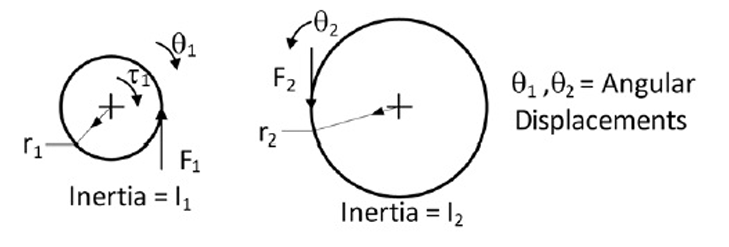
\includegraphics[width=0.5\textwidth]{Fig 17.png}
\caption{}
\label{fig:question51}
\end{figure}

\begin{enumerate}
    \item $ F_1 \neq F_2 $; $ \tau_1 = I_1 \theta_1 $; $ F_2 = I_2 \frac{r_1}{r_2^2} \theta_1 $
    \item $ F_1 = F_2 $; $ \tau_1 = \left[ I_1 + I_2 \left( \frac{r_1}{r_2} \right)^2 \right] \theta_1 $; $ F_2 = I_2 \frac{r_1}{r_2^2} \theta_1 $
    \item $ F_1 = F_2 $; $ \tau_1 = I_1 \theta_1 $; $ F_2 = I_2 \frac{1}{r_2} \theta_2 $
    \item $ F_1 \neq F_2 $; $ \tau_1 = \left[ I_1 + I_2 \left( \frac{r_1}{r_2} \right)^2 \right] \theta_1 $; $ F_2 = I_2 \frac{1}{r_2} \theta_2 $
\end{enumerate}
\hfill  (GATE ME 2015)

\item A mobile phone has a small motor with an eccentric mass used for vibrator mode. The location of the eccentric mass on motor with respect to center of gravity (CG) of the mobile and the rest of the dimensions of the mobile phone are shown. The mobile is kept on a flat horizontal surface.

\begin{figure}[H]
\centering
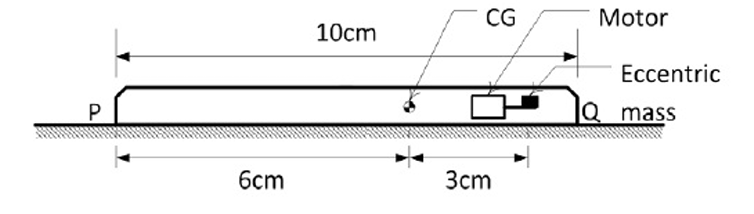
\includegraphics[width=0.5\textwidth]{Fig 18.png}
\caption{}
\label{fig:question52}
\end{figure}

Given in addition that the eccentric mass = 2 grams, eccentricity = 2.19 mm, mass of the mobile = 90 grams, $ g = 9.81 \, \text{m/s}^2 $. Uniform speed of the motor in RPM for which the mobile will get just lifted off the ground at the end Q is approximately

\begin{multicols}{4}
\begin{enumerate}
    \item 3000
    \item 3500
    \item 4000
    \item 4500
\end{enumerate}
\end{multicols}
\hfill  (GATE ME 2015)

\item A machine element is subjected to the following bi-axial state of stress: $\sigma_x = 80 \, \text{MPa}; \sigma_y = 20 \, \text{MPa}; \tau_{xy} = 40 \, \text{MPa}$. If the shear strength of the material is 100 MPa, the factor of safety as per Tresca’s maximum shear stress theory is

\begin{multicols}{4}
\begin{enumerate}
    \item 1.0
    \item 2.0
    \item 2.5
    \item 3.3
\end{enumerate}
\end{multicols}
\hfill  (GATE ME 2015)

\item A cantilever beam with flexural rigidity of $200 \, \text{Nm}^2$ is loaded as shown in the figure. The deflection (in mm) at the tip of the beam is -------------.

\begin{figure}[H]
\centering
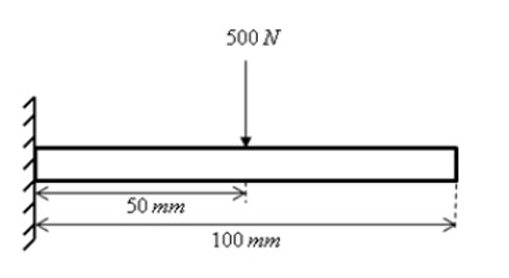
\includegraphics[width=0.5\textwidth]{Fig 19.png}
\caption{}
\label{fig:question54}
\end{figure}
\hfill  (GATE ME 2015)

\item A precision instrument package ($m = 1 \, \text{kg}$) needs to be mounted on a surface vibrating at $60 \, \text{Hz}$. It is desired that only 5\% of the base surface vibration amplitude be transmitted to the instrument. Assume that the isolation is designed with its natural frequency significantly lesser than $60 \, \text{Hz}$, so that the effect of damping may be ignored. The stiffness (in N/m) of the required mounting pad is -------------.

\hfill  (GATE ME 2015)

\item A horizontal plate has been joined to a vertical post using four rivets arranged as shown in the figure. The magnitude of the load on the worst loaded rivet (in N) is -------------.

\begin{figure}[H]
\centering
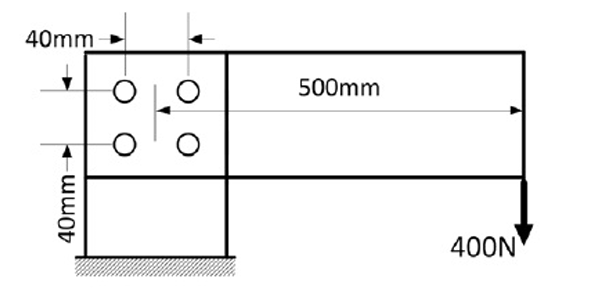
\includegraphics[width=0.5\textwidth]{Fig 20.png}
\caption{}
\label{fig:question56}
\end{figure}
\hfill  (GATE ME 2015)

\item For flow through a pipe of radius $ R $, the velocity and temperature distribution are as follows:
$ u(r, x) = C_1 $
and 
$ T(r, x) = C_2 \left[ 1 - \left( \frac{r}{R} \right)^3 \right] $
where $ C_1 $ and $ C_2 $ are constants.
The bulk mean temperature is given by 
$ T_m = \frac{2}{U_m R^2} \int_0^R u(r, x) T(r, x) r \, dr $
with $ U_m $ being the mean velocity of flow. The value of $ T_m $ is

\begin{multicols}{4}
\begin{enumerate}
    \item $\frac{0.5C_2}{U_m}$
    \item $0.5C_2$
    \item $0.6C_2$
    \item $\frac{0.6C_2}{U_m}$
\end{enumerate}
\end{multicols}
\hfill  (GATE ME 2015)

\item Match the following pairs:

\begin{tabular}{|c|c|c|c|}
\hline
 & Equation & & Physical Interpretation \\
\hline
P & $ \nabla \times \vec{V} = 0 $ & I & Incompressible continuity equation \\
\hline
Q & $ \nabla \cdot \vec{V} = 0 $ & II & Steady flow \\
\hline
R & $ \frac{D\vec{V}}{Dt} = 0 $ & III & Irrotational flow \\
\hline
S & $ \frac{\partial \vec{V}}{\partial t} = 0 $ & IV & Zero acceleration of fluid particle \\
\hline
\end{tabular}

\begin{enumerate}
    \item P-IV, Q-I, R-II, S-III
    \item P-IV, Q-III, R-I, S-II
    \item P-III, Q-I, R-IV, S-II
    \item P-III, Q-I, R-II, S-IV
\end{enumerate}
\hfill  (GATE ME 2015)

\item The velocity field of an incompressible flow is given by
$ \vec{V} = (a_1 x + a_2 y + a_3 z)\vec{i} + (b_1 x + b_2 y + b_3 z)\vec{j} + (c_1 x + c_2 y + c_3 z)\vec{k} $, where $ a_1 = 2 $ and $ c_3 = -4 $. The value of $ b_2 $ is -------------.

\hfill  (GATE ME 2015)

\item A 10 mm diameter electrical conductor is covered by an insulation of 2 mm thickness. The conductivity of the insulation is 0.08 W/m-K and the convection coefficient at the insulation surface is 10 W/m$^2$-K. Addition of further insulation of the same material will

\begin{enumerate}
    \item increase heat loss continuously
    \item decrease heat loss continuously
    \item increase heat loss to a maximum and then decrease heat loss
    \item decrease heat loss to a minimum and then increase heat loss
\end{enumerate}
\hfill  (GATE ME 2015)

\item Temperature of nitrogen in a vessel of volume 2 m$^3$ is 288 K. A U-tube manometer connected to the vessel shows a reading of 70 cm of mercury (level higher in the end open to atmosphere). The universal gas constant is 8314 J/kmol-K, atmospheric pressure is 1.01325 bar, acceleration due to gravity is 9.81 m/s$^2$ and density of mercury is 13600 kg/m$^3$. The mass of nitrogen (in kg) in the vessel is -------------.

\hfill  (GATE ME 2015)

\item Air ($\rho = 1.2 \, \text{kg/m}^3$ and kinematic viscosity, $\nu = 2 \times 10^{-5} \, \text{m}^2/\text{s}$) with a velocity of 2 m/s flows over the top surface of a flat plate of length 2.5 m. If the average value of friction coefficient is $C_f = \frac{1.328}{\sqrt{Re_x}}$, the total drag force (in N) per unit width of the plate is -------------.

\hfill  (GATE ME 2015)

\item Water ($\rho = 1000 \, \text{kg/m}^3$) flows through a venturimeter with inlet diameter 80 mm and throat diameter 40 mm. The inlet and throat gauge pressures are measured to be 400 kPa and 130 kPa respectively. Assuming the venturimeter to be horizontal and neglecting friction, the inlet velocity (in m/s) is -------------.

\hfill  (GATE ME 2015)

\item A well insulated rigid container of volume $1 \, \text{m}^3$ contains 1.0 kg of an ideal gas [$C_p = 1000 \, \text{J/(kg.K)}$ and $C_v = 800 \, \text{J/(kg.K)}$] at a pressure of $10^5 \, \text{Pa}$. A stirrer is rotated at constant rpm in the container for 1000 rotations and the applied torque is 100 N-m. The final temperature of the gas (in K) is -------------.

\hfill  (GATE ME 2015)

\item Steam enters a well insulated turbine and expands isentropically throughout. At an intermediate pressure, 20 percent of the mass is extracted for process heating and the remaining steam expands isentropically to 9 kPa.

Inlet to turbine: $P = 14 \, \text{MPa}, T = 560^\circ\text{C}, h = 3486 \, \text{kJ/kg}, s = 6.6 \, \text{kJ/(kg.K)}$ \\
Intermediate stage: $h = 2776 \, \text{kJ/kg}$ \\
Exit of turbine: $P = 9 \, \text{kPa}, h_f = 174 \, \text{kJ/kg}, h_g = 2574 \, \text{kJ/kg}, s_f = 0.6 \, \text{kJ/(kg.K)}, s_g = 8.1 \, \text{kJ/(kg.K)}$

If the flow rate of steam entering the turbine is 100 kg/s, then the work output (in MW) is -------------.

\hfill  (GATE ME 2015)


\end{enumerate}
\end{document}
